\documentclass[UKenglish]{ifimaster}  %% ... or USenglish or norsk or nynorsk
\usepackage[utf8]{inputenc}           %% ... or latin1 or applemac
\usepackage[T1]{fontenc,url}
\urlstyle{sf}

\usepackage[dvipsnames,svgnames,table]{xcolor} 	% must come before various stuff
															% dont know what, but many packages
															% include color.

\usepackage{textcomp}

\usepackage{csquotes}

\usepackage{ifimasterforside}


\usepackage{varioref} 	% Must be included before hyperref

\usepackage[bookmarks,breaklinks,pdfpagelabels,
urlcolor=black,
colorlinks=true,  % Colors links instead of ugly boxes
urlcolor=blue,    % Color for external hyperlinks
linkcolor=black,  % Color of internal links
citecolor=black,  % Color of citations
linktoc=all,
plainpages=false,
%pagebackref=true,
%backref=true,
%hyperindex=false,
urlcolor=black]{hyperref}   % Reference package, must be before cleveref

\usepackage[all]{hypcap}    % Link to figures (\ref{label}) go to the image,
                            % and not the caption (Default value is true)
							
\usepackage[noabbrev]{cleveref}[2013/12/28] % Provides \cref command (must be after hyperref)  
											% When use e.g \crefname{tcb@cnt@tablebox}{table}{tables}
											% a \cref will automatically write table/figure etc.


\usepackage{graphicx}
\usepackage[norsk, english]{babel}


\usepackage{caption}
\usepackage{subcaption}

\usepackage{float}
\usepackage{newfloat}   % Used for the custom listings (listofcodelistings, listofcommands)

\usepackage{booktabs}

\usepackage[most]{tcolorbox}[2014/05/28] % Minimum v3.05
\tcbuselibrary{most}
\tcbuselibrary{listings}
\tcbuselibrary{breakable}
\tcbuselibrary{skins}
\usetikzlibrary{shadings}

%
% Declare a new floating type for the Source Code
%
\DeclareFloatingEnvironment[
  fileext=loc,
  listname={List of Source code listings},
  name=Code Listing,
  placement=htp,
]{codelisting}

\makeatletter % Must change the catcode of @ to 11 before defining the listing style

% add tcblistings to \jobname.loc (list of codes)
\tcbset{
  listingcaption/.store in=\kvtcb@listingcaption,%
   addtolol/.style={list entry={\numberline {\thetcbcounter}%
       {\ignorespaces \kvtcb@listingcaption}},%
     add to list={loc}{section}},
}

%%%%%%%%%%%%%%%%%%%%%%
%% Code listing style
%%%%%%%%%%%%%%%%%%%%%%

%\newcommand{\codecommentcolor}{\color{yellow!50!red}}
\colorlet{codecommentcolor}{yellow!50!red}

% language and style definition
\lstdefinestyle{Cppstyle}
{%
  language = C++,
  basicstyle=\footnotesize\ttfamily,
  keywordstyle=\bfseries\color{green!40!black},
  identifierstyle=\color{blue},
  % keywordstyle=\bfseries\color{green!40!black},
  commentstyle=\itshape\color{purple!40!black},
  stringstyle=\color{orange},
  %morecomment=[l][\color{yellow!50!red}]{//},
  morecomment=[l][\color{codecommentcolor}]{//},
  %morecomment=[l][\codecommentcolor{}]{//},
  %escapechar=@,
  %morecomment=[s][\color{green}]{/*}{*/},
  %keywordstyle = \color{blue},
}[keywords,strings,comments]

%%%%%%%%%%%%%%%%%%%%%%
%% Code listing
%%%%%%%%%%%%%%%%%%%%%%

\newtcblisting[auto counter,
number within=chapter,
]{cppcode}[1][]{%
  listing only,
  %colback=white,
  %colback=red!30!white,
  colback=lightgray!10!white,
  %colbackmiddlefirst=!88!black,
  %colbackmiddlelast=!93!black,
  %colback=lightgray!40!white,
  %colbackmiddlefirst=!40!white,
  %colbackmiddlelast=!40!white,
  %colback=white,
  %colbackmiddlefirst=!40!white,
  %colbackmiddlelast=!40!white,
  %colbacklower=white,
  colframe=gray!60!white,
  fontlower=\small,
%  listing remove caption=true,
  %skin=beamercustom,
  lower separated=true,
  listing engine=listings,
  breakable,
  enlarge top by=0.5cm,          % Add space above the box
%  enlarge top by=1cm, % Add space before the code listing
%  enlarge bottom by=0.3cm, % Add space after the code listing
  arc=0cm,            % Remove the rounded corners
  outer arc=0.3mm,    % Remove the rounded corners on outside
%
  % Add space on left side of content. This moves the line numbering inside the box
  left=8mm,
%
  top=0pt,
  bottom=0pt,
%
  boxrule=0mm,        % The border width
  bottomrule=0.7pt,
  leftrule=0.7pt,
  rightrule=1pt,
  lines before break=6, % Require at least 5 lines in the upper part to break the code block
                        % If less than 5, the code block is moved to next page.
% boxrule=0.7pt,        % The border width
%
  toptitle=2pt,       % Add space in title bar
  bottomtitle=1pt,    % Add space in title bar
  title={Source Code \thetcbcounter}, % Set default box title to
  %listingcaption=\kvtcb@title,    % Set default code list title to box title
  listing options={
    style=Cppstyle,
    breaklines=true,
    numbers=left,
  },
  #1,
}

\crefname{tcb@cnt@cppcode}{code listing}{code listings}
\Crefname{tcb@cnt@cppcode}{Code listing}{Code listings}



%%%%%%%%%%%%%%%%%%%%%%
%% Tables box
%%%%%%%%%%%%%%%%%%%%%%
\newtcolorbox
  {tablebox}[1][]{%
  title={Table \thetcbcounter}, % Set default box title
  top=5mm,                       % Add space between title and content
  left=0mm,
  right=0mm,
  colback=white,
  toptitle=1pt,
  bottomtitle=0pt,
  %colframe=blue!40!white,
  colframe=DodgerBlue!60!white,
  enlarge top by=0.5cm, % Add space before the table
  arc=0cm,            % Remove the rounded corners
  outer arc=0.3mm,    % Remove the rounded corners on outside
  #1,
}

\crefname{tcb@cnt@tablebox}{table}{tables}
\Crefname{tcb@cnt@tablebox}{Table}{Tables}


%%%%%%%%%%%%%%%%%%%%%%
%% Figures box
%%%%%%%%%%%%%%%%%%%%%%
\newtcolorbox[auto counter,
number within=chapter,
%crefname={figure}{Figure},
%Crefname={Figure}{Figures},
]{figurebox}[1][]{%
  title={Figure \thetcbcounter}, % Set default box title
 % enhanced,
  %minipage boxed title=7.5cm,
 % attach boxed title to top center,
%  enlarge top by=0.5cm,         % Floats have a default spacing, so no need to set this for figures
  top=5mm,                       % Add space between title and content in the box
  toptitle=1pt,
%  boxrule=0.7pt,        % The border width
  boxrule=0.0pt,        % The border width
  bottomrule=0mm,
  colback=white,                 % Background color
%  boxsep=0mm,
 % colframe=Firebrick4!60!white,
  %colframe=black!75!white,
 % colframe=figureframecolor,
%x  coltitle=Firebrick4!90!white,
%  center title,
 colframe=white,
  arc=0cm,                       % Remove the rounded corners
%  outer arc=0.3mm,               % Remove the rounded corners on outside
  #1,
}
\crefname{tcb@cnt@figurebox}{figure}{figures}
\Crefname{tcb@cnt@figurebox}{Figure}{Figures}

\crefname{subfigure}{subfigure}{subfigures}
\Crefname{subfigure}{Subfigure}{Subfigures}


% Must be defined here, apparently
\def\@captype{codelisting}

\newcommand{\codebox}[1]{\capstart\begin{cppcode}[#1]}

\AtBeginDocument{%
  \NewDocumentCommand{\boxcaption}{mmO{#2}}{\begingroup \captionof{#1}[#3]{#2} \endgroup}
}

\makeatother % changes the catcode of @ back to 12

\include{tex_extensions/colours}



\makeatletter % Must change the catcode of @ to 11 before defining the listing style
\newcommand{\addchaptolistof}[2]{% arg1=type, arg2=listname
\newtoggle{#1chapbool}
\pretocmd{\Hy@org@chapter}{\global\toggletrue{#1chapbool}}{}{}
\pretocmd{\caption}{%
  \iftoggle{#1chapbool} {
    \ifthenelse{\equal{#1}{\@captype}}{
      \addtocontents{#2}{\vskip\bigskipamount\noindent\textbf{Chapter \thechapter%\argone
        }\par\nobreak\vskip\medskipamount}
      \global\togglefalse{#1chapbool}%
    }{}%
  }{}%
}{}{}
}
\makeatother % changes the catcode of @ back to 12
  % Make listof categorized by chapter
\usepackage[colorinlistoftodos
%,disable
]{todonotes}
\setlength{\marginparwidth}{3cm}

%%%%%%%%%%%%%%%%%%%%%%%%%%%%%%%%%%%%%%%%%%%%%%%%%%%
%% This file defines a few different todo commands:
%%
%% \feedback, \atodo, \citeneeded which are different
%% variations of \todo with color and title
%%
%% Make list of todos with \insertlistoftodos
%%
%%%%%%%%%%%%%%%%%%%%%%%%%%%%%%%%%%%%%%%%%%%%%%%%%%%

%
% Change the title of the todo list if needed
%
\newcommand{\todolisttitle}{Todo list}
\newcommand{\debugprint}{DEBUGING}

\newcommand{\insertlistoftodos}{%
% Add TODO list
\newpage
\phantomsection % Sets correct page reference link for the code listings
\hypertarget{todolistref}{}
\bookmark[dest=todolistref,level=0]{\todolisttitle}
% Use the line below to add entry to table of contets. (Remember to comments out the line above)
%\addcontentsline{toc}{chapter}{\protect\numberline{}{\todolisttitle}}
\listoftodos
}

\newtoggle{todoChapToggle}
\newtoggle{todoSectToggle}

\makeatletter % Must change the catcode of @ to 11 before defining the listing style
% Set todo list title
\@todonotes@SetTodoListName{\todolisttitle}%

% Reset todoChapToggle and todoSectToggle at chapter/section start
\pretocmd{\Hy@org@chapter}{\global\toggletrue{todoChapToggle}}{}{}
\pretocmd{\section}{\global\toggletrue{todoSectToggle}}{}{}
\makeatother % changes the catcode of @ back to 12

% Creating a missing reference todo command
\newcounter{todorefcounter}
\newcommand{\atodo}[2][]{\addtocounter{todorefcounter}{1}%
  \todo[%color=red!40,%
  caption={\protect\hypertarget{todo\thetodorefcounter}{}Todo \thetodorefcounter: #2},%
  #1]{\thetodorefcounter: Todo\\ #2. \hyperlink{todo\thetodorefcounter}{$\uparrow$}
  }
}

\newcounter{citeneededfcounter}
\newcommand{\citeneeded}[2][]{\addtocounter{citeneededfcounter}{1}\todo[color=red!40,%
  caption={\protect\hypertarget{citeneeded\theciteneededfcounter}{}Citation needed \theciteneededfcounter: #2},%
  #1]{Citation needed: \theciteneededfcounter\\ #2. \hyperlink{citeneeded\theciteneededfcounter}{$\uparrow$}
  }
}

\newcounter{commentcounter}
\newcommand{\acomment}[2][]{\addtocounter{commentcounter}{1}\todo[color=red!40,%
  caption={\protect\hypertarget{comment\thecommentcounter}{}Comment \thecommentcounter: #2},%
  #1]{Comment: \thecommentcounter\\ #2. \hyperlink{comment\thecommentcounter}{$\uparrow$}
  }
}

\newcounter{todofeedbackcounter}
\DeclareDocumentCommand{\feedback}{ O{} O{} m }{
\addtocounter{todofeedbackcounter}{1}\todo[color=yellow!40,%
author={\thetodofeedbackcounter: Feedback}, %
caption={\protect\hypertarget{feedback\thetodofeedbackcounter}{}Feedback \thetodofeedbackcounter: #3},%
  #1]{\ifx&#2&%
    \else
    {\color{blue}~#2:}
   \fi
   \\ #3. \hyperlink{feedback\thetodofeedbackcounter}{$\uparrow$}
 }}

\newcounter{questioncounter}
\DeclareDocumentCommand{\question}{ O{} O{} m }{
\addtocounter{questioncounter}{1}\todo[color=green!40,%
  caption={\protect\hypertarget{question\thequestioncounter}{}Question \thequestioncounter: #3},%
  #1]{\thequestioncounter: Question
    \ifx&#2&%
    \else
    {\color{blue}~#2:}
   \fi
   \\ #3. \hyperlink{question\thequestioncounter}{$\uparrow$}
 }}



% This handles adding the chapter/section to the todo notes list
\pretocmd{\atodo}{%
  \iftoggle{todoChapToggle}{
    \addtocontents{tdo}{%
      \vskip\bigskipamount\noindent\textbf{\LARGE{Chapter \thechapter}}\par\nobreak\vskip\medskipamount}
    \global\togglefalse{todoChapToggle}%
  }{}%
  \iftoggle{todoSectToggle}{%
    \addtocontents{tdo}{%
      \vskip\bigskipamount\noindent\textbf{\large{Section \thesection}}\par\nobreak\vskip\medskipamount}
    \global\togglefalse{todoSectToggle}
  }{}
}{}{}


\AtBeginDocument{%
  % Add the lists to categorize
  \addchaptolistof{figure}{lof}
  \addchaptolistof{table}{lot}
  \addchaptolistof{codelisting}{loc}
}


\title{The title of my thesis}       
\subtitle{Any short subtitle}        
\author{Kristian Skarseth}  

\begin{document}
\ififorside{}
\frontmatter{}
\maketitle{}

\chapter*{Abstract}                  

\tableofcontents{}
\listoffigures{}
\listoftables{}
\listofcodelistings

\chapter*{Preface}                  
Would like to thank Bendik Rønning Opstad for his help with Latex. 
\mainmatter{}

%%%%=========================================%%%%
%%%%=========================================%%%%
%%%%=========================================%%%%
\part{Introduction}        
%%%%=========================================%%%%
%%%%=========================================%%%%
%%%%=========================================%%%%
           
\chapter{Introduction}\label{chap:intro}

%%%%%%%%%%%%%%%%%%%%%%%%%%%%%%%%%%%%%%%%%%%%%%%%%%%%%%%%%%%%%%%%%%%
%%%%%%%%%%%%%%%%%%% I N T R O D U C T I O N %%%%%%%%%%%%%%%%%%%%%%%
%%%%%%%%%%%%%%%%%%%%%%%%%%%%%%%%%%%%%%%%%%%%%%%%%%%%%%%%%%%%%%%%%%%
\section{Introduction}\label{sect:intro}
Today there are no open source and free to use implementations of an accepted standard for full reference objective video quality assessment. In this paper we present the preliminary work for what will be an open source and free to use implementation of OPTICOMs PEVQ model \cite{j.247}. We will also provide an introduction to the history of digital video quality assessment, including validation test results for various full reference (FR), reduced reference (RR) and no reference (NR) assessment methods which is the basis for our reasoning behind choosing the PEVQ model. Finally we present the current progress of our implementation of PEVQ, including some preliminary results and an outline for future work.


\subsection{Background}\label{sect:background}
From the time digital video codecs became widely used in the early 1990s there has been a demand for ways to objectively assess the quality of encoded video. Relying on subjective quality assessment is both time consuming and expensive, while a tool for objective quality assessment would be able to reduce both the cost and the time of measuring the quality of the video. The necessity for such a tool has been acknowledged by many, and today several standards for objective video quality assessment have been written.


\subsection{Problem Definition and goals}\label{sect:problem}
As we will show in this paper, much work has been done towards creating an objective video quality assessment tool that can be as accurate as a well designed subjective test. The latest of such tools that provide the best results and resolution support are implemented and copyrighted by various companies, making it too expensive for most researchers and other potential users to benefit from using the software. Instead these users are forced to use less accurate tools which may be cheaper or free. This has motivated us to find and create our own free to use and open implementation of the best available open standard. It is also our goal to submit our solution to VLC\cite{vlc} and have it incorporated in their group of video handling software in order to make it easily and widely accessible.


\subsection{Outline}\label{sect:outline}
In section~\ref{sect:history} we present the history behind video quality assessment. Section~\ref{sect:ovqa} describes the various objective quality assessment approaches in detail. Section~\ref{sect:cts} provides the arguments and reasoning behind choosing the PEVQ model, as well as a brief explanation of the model itself. Section~\ref{sect:implementation} showcases the current implementation and preliminary results, and section~\cref{sect:summary} presents a summary of the paper, as well as a separate summary of possible future work.

%%%%%%%%%%%%%%%%%%%%%%%%%%%%%%%%%%%%%%%%%%%%%%%%%%%%%%%%%%%%%%%%%%%
%%%%%%%%%%%%%%%%%%%%%%%% H I S T O R Y  %%%%%%%%%%%%%%%%%%%%%%%%%%%
%%%%%%%%%%%%%%%%%%%%%%%%%%%%%%%%%%%%%%%%%%%%%%%%%%%%%%%%%%%%%%%%%%%
\section{History}\label{sect:history}

Following digital video codecs becoming more and more mainstream in the early 1990s, a big challenge was, and still is, to create codecs that provide the optimal ratio of video quality and data quantity, and to find the best way of streaming digitally encoded video sequences over the Internet. For codecs, the correct ratio will depend on the use case. You may accept a higher data quantity for an increased video quality when you store the original of a video clip. However you may also have to live with lower quality in order to reduce the data quantity when streaming the video over the internet. 

Testing the quality of the video, especially after the video sequence comes out on the other end of a streaming procedure, is an important step in both finding the correct codec and especially the correct streaming protocol. Producing a subjective test score relies on well designed and organized tests with several test subjects. Performing such a test will likely be both expensive and time consuming. On the other hand, a tool for producing an objective quality assessment score could be able to rate the quality of the video faster, cheaper and without the involvement of large subjective testing groups. Researchers with access to such a tool would be in a good position when testing anything they are developing that handles and\slash or alters video sequences.

\subsection{Peak Signal to Noise Ratio}\label{sect:psnr}
A much used approach to testing video quality objectively is Peak Signal to Noise Ratio (PSNR). It is simple, and has been used for a long time. However, when the original video content is altered in any way, the quality measured by PSNR is not reliably close to the assessment results coming from subjective testing. A better approach is taking the human visual system (HVS) into account when analysing the video quality. This is explained, among others, by Huynh-Thu and M. Gihanbari in \cite{4550695} and Bernd Giron in\cite{Girod:1993:WWM:197765.197784}.

\subsection{Validation of Perceptual Objective Video Quality Assessment standards}\label{sect:validation}
Unlike PSNR, perceptual objective video quality assessment tools attempt to mimic the HVS so that the results may be closer to subjective test results. In order to meet requirements and expectations from users for a potential objective video quality assessment tool, a subcommittee of The American National Standards Association (ANSI), named Accredited Alliance for Telecommunications Industry Solution (ATIS), performed a validation test for objective video quality measurement. As described by Pinson, Staelens and Webster in\cite{6659332}, the report\cite{T1A1.5} from the testing, performed by the group T1A1.5 within ATIS, laid the groundwork for future tests of objective video quality assessment tools. Two standards were also formed after the testing, the ANSI Standard T1.801.03 and T1.801.01. The following information is based on a paper by Pinson, Staelens and Webster\cite{6659332}, summarizing the history of video quality model validation.

In 1997 the first meeting of the Video Quality Experts Group (VQEG, www.vqeg.org) found place in Turin. VQEG was formed so that international experts within subjective video quality measurement could come together and share their information. The purpose of the group was and still is to advance within the field of video quality assessment.

To date the VQEG group has gone through several large testing phases. From 1999 to 2000 their first phase, called the full reference television (FRTV) phase I, were conducted by the Independent Lab Group (ILG). It was designed for testing objective full- and no-reference standard definition television quality; however none of the no reference models made it to the testing phase. The conclusion from the test was that none of the submitted models were statistically better than PSNR.

Following the FRTV phase I came FRTV phase II (2002-2003), the multimedia phase I (2007-2008), reduced reference/no reference television (RRNR-TV) phase I (2008-2009) and the high definition television (HDTV) test (2009-2010, all tests conducted by ILG with some proponents involved in certain cases. Eight full reference FR models were published in a first rendition of ITU-T Rec. J144 following FRTV phase I (2001), and FRTV phase II published a revised version of ITU-T Rec. J144 as well as ITU-T Rec. BT.1683, where two FR models were standardized. In both phases all no reference (NR) models were withdrawn. Following the multimedia phase I, FR models from Nippon Telegraph and Telephone Corporation (NTT), OPTICOM, Psytechnics and Yonsei University were standardized in ITU-T Rec. J.247 and ITU-R BT.1866. A reduced reference (RR) model from Yonsei University was standardized in ITU-T Rec. J.246 and ITU-R BT.1867. Again no NR models were standardized. The RRNR-TV phase I test standardized 3 RR models in ITU-T Rec. J.249, and the HDTV test in 2009-2010 standardized two FR models in J.341 and a RR models in J.242. Two NR models were mentioned in VQEGs final report for the HDTV test, but neither was standardized. For more information on the history of VQEGs validation tests, see Staelens and Websters paper in\cite{6659332}.

\begin{table}
	%\center
	\begin{tablebox}[adjusted title= Overview of test phases, width=\linewidth]
	%\footnotesize
	\resizebox{\textwidth}{!}{%
	%\caption{Overview of test phases}
    \begin{tabular}{p{3cm}p{1.5cm}p{2cm}p{3cm}p{5cm}}
    Test-phase name  & Org. & Date      & Resolutions      & Standards documents                                                \\
    \toprule
    T1A1            & ATIS & 1994-1995 & NTSC             & T1.801.03 \& T1.801.01                                             \\
    FRTV Phase I    & VQEG & 1999-2000 & NTSC \& PAL      & ITU-T Rec. J.144                                                   \\
    FRTV Phase II   & VQEG & 2002-2003 & NTSC \& PAL      & ITU-T Rec. J.144 \& ITU-R Rec. BT.1683                             \\
    Multimedia      & VQEG & 2007-2008 & VGA, CIF \& QCIF & ITU-T Rec. J.247, ITU-R BT.1866, ITU-T Rec. J.246 \& ITU-R BT.1867 \\
    RRNR-TV Phase I & VQEG & 2008-2009 & NTSC \& PAL      & ITU-T Rec. J.249                                                   \\
    HDTV            & VQEG & 2009-2010 & 1080i \& 1080p   & ITU-T Rec. J.341 \& ITU-T Rec. J.242                               \\
    \end{tabular}	
    }
    \end{tablebox}
    \caption{Overview of test phases}
	\label{table:testOverview}
\end{table}

Table \ref{table:testOverview} shows a summary of the test phases we have talked about with the name of the test phase, name of the organization who designed the test, the date, tested resolutions and standards documents for objective video quality assessment published following the tests.

In order to further improve and advance the field of validation of video quality metrics, VQEG have also started the Joint Effort Group (JEG) which is developing tools and laying a groundwork for others who wish to validate video quality metrics. More about the JEG group can be read in Staelens et. al. paper\cite{6065713}.

In the next section we will provide an introduction to exactly what objective video quality assessment means, and the difference between the three approaches mentioned in this section, no-, reduced- and full-reference objective video quality assessment.

%%%%%%%%%%%%%%%%%%%%%%%%%%%%%%%%%%%%%%%%%%%%%%%%%%%%%%%%%%%%%%%%%%%
% O B J E C T I V E  V I D E O  Q U A L I T Y  A S S E S S M E N T 
%%%%%%%%%%%%%%%%%%%%%%%%%%%%%%%%%%%%%%%%%%%%%%%%%%%%%%%%%%%%%%%%%%%
\section{Objective video quality assessment}\label{sect:ovqa}
As we have been able to see from the history of objective video quality assessment, the approach with highest consistency compared to the subjective counterpart is the full reference (FR) version. This is however also the approach that requires the most background data for any video sequence in order to give results. The reduced reference (RR) and no reference (NR) methods can be executed without access to the full source material. In order to better understand our decision to choose a FR model the next three sections will give an overview of the three approaches to objective video quality assessment. To read more about the differences to the methods mentioned in the following three sections you can see S. Chikkerur and V. Sundarams paper in\cite{5710601}.

%missing a reliable/good source for the sections
\subsection{No reference objective video quality assessment}\label{sect:nr}
NR points to the fact that there is no reference to the original source material when measuring and determining the quality of the video. This means that the assessment is done purely by analysing the degraded signal. In an environment where there is no access to any source material the only possible objective approach will be a NR method. However as we could see in section~\ref{sect:history} the performance of NR methods are to this date significantly lower compared to that of RR and FR approaches.


\subsection{Reduced Reference objective video quality assessment}\label{sect:rr}
RR is a middle ground between NR and FR in that it has access to certain information about the source signal. The information can be transmitted where there is limited transmission capacity and therefore limited access to the reference signal. This limited extra information about the source signal can still be enough to provide better results than a NR approach, and as we saw in section~\ref{sect:history} several standards have been approved for RR methods. 

%as could be seen in history this has some better accuracy, and standard(s?) have been approved.

\subsection{Full Reference objective video quality assessment}\label{sect:fr}
FR is the final approach where the entire source signal is available together with the degraded signal. This means we can compare the two signals as detailed as on a per pixel basis and draw a conclusion from the difference between the two signals. Considering all data is available during the measurement it makes sense that a FR technique will be most accurate, and as we could see from section~\ref{sect:history} this has also been the case in tests designed by VQEG. 

%%%%%%%%%%%%%%%%%%%%%%%%%%%%%%%%%%%%%%%%%%%%%%%%%%%%%%%%%%%%%%%%%%%
%%%%%%%%%% C H O O S I N G  T H E  S T A N D A R D  %%%%%%%%%%%%%%%
%%%%%%%%%%%%%%%%%%%%%%%%%%%%%%%%%%%%%%%%%%%%%%%%%%%%%%%%%%%%%%%%%%%

\section{Choosing the standard}\label{sect:cts}

It was important to us to choose an approved standard when implementing an open and free to use solution. If anyone is to rely on the tool we create they must be able to trust that it gives results at least close to that of other tools you can purchase. Selecting one of the models standardized through VQEG testing was therefore a natural choice. After taking that decision we had to choose between a NR, RR and FR model. To date no NR models have been standardized, as shown in section~\ref{sect:history}, which makes it easy to dismiss any such models. The choice between RR and FR models has come came down to choosing the open standard that can be implemented without paying royalties, while also having performed very well in testing. We have chosen OPTICOMs PEVQ model which was standardized in ITU-T Rec. J.247\cite{j.247}. Three other models were also available in this standard, but the OPTICOM model scored overall best which can be seen in \cref{table:subjCorr}. The tables use values from the J.247 standard, where the correlation values represent how closely the results from each model correlates with subjective test results. The closer to 1 the correlation value is, the better is the result.






\begin{table}[h]

\begin{tablebox}[adjusted title= Subjective test result correlation,%
width=\linewidth]
%\footnotesize
\resizebox{\textwidth}{!}{%
 
\begin{tabular}{@{}lllllllllll@{}}

& \multicolumn{2}{c}{NIT} 
& \multicolumn{2}{c}{OPTICOM} 
& \multicolumn{2}{c}{Psytechnics} 
& \multicolumn{2}{c}{Yonsei} 
& \multicolumn{2}{c}{PSNR} \\ 
& $C_{avg}$ & $C_{min}$ & $C_{avg}$ & $C_{min}$ & $C_{avg}$ 
& $C_{min}$ & $C_{avg}$ & $C_{min}$ & $C_{avg}$ & $C_{min}$ \\ 
\toprule
VGA  & 0.786 & 0.598 & 0.825 & 0.685 & 0.822 & 0.565 & 0.805 & 0.612 & 0.713 & 0.499 \\
CIF  & 0.777 & 0.675 & 0.808 & 0.695 & 0.836 & 0.769 & 0.785 & 0.712 & 0.656 & 0.440 \\
QCIF & 0.819 & 0.711 & 0.841 & 0.724 & 0.830 & 0.664 & 0.756 & 0.587 & 0.662 & 0.540 \\ 
%\bottomrule
\end{tabular}
}
\end{tablebox}

\caption[Subjective test correlation for the models tested in J.247, also including PSNR.]%
{Subjective test correlation for the models tested in J.247, also including PSNR. $C_{avg}$ and $C_{min}$ represents avg. correlation and min. correlation. \cite{j.247}}%
\label{table:subjCorr}
\end{table}

The biggest limitation of the PEVQ model from ITU-T Rec. J.247 is the tested resolutions which are limited to VGA, CIF and QCIF. HD resolution is Today in full use in most applications, and choosing a standard which is not designed for HD seems strange. This is unfortunately a limitation we have to accept as the models described in newer standards, such as ITU-T Rec. J.341, that does support HD, have been patented in such a way that we cannot make our own implementation for free. 

\subsection{Description of PEVQ}\label{sect:pevq}
PEVQ as standardized in ITU-T Rec. J.247 is a FR objective video quality assessment model designed to measure video quality on mobile and multimedia platforms. It does so by calculating five indicators, each operating in different domains (temporal, spatial, luminance and chrominance) motivated by the human visual system (HVS) so that it may attempt to see the video as a human subject would. The model requires two input signals, the full reference (source) signal and the full degraded signal. The model will go through several stages where both signals are processed and results from the processing stages are weighted together to provide the final result.

\begin{figure}[h]
	  \centering
	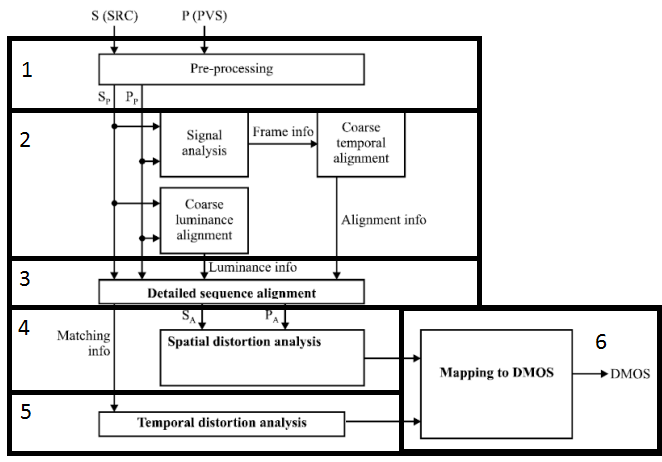
\includegraphics[width=0.7\textwidth,natwidth=662,natheight=588]{images/pevqOverview.png}
	\caption{Overview of the PEVQ model.}
	\label{fig:pevqOverview}
\end{figure}
	  
Using figure~\ref{fig:pevqOverview} we describe the basic flow of PEVQ. The first stage consists pre-processing where a spatial region of interest (RIO) is extracted from the two signals. The RIO is the area on the video where all the following processing will be performed, while the leftover edges are used only for certain calculations where neighbour pixel-data is required. Following the RIO extraction comes a coarse alignment registration of the input sequences which in step 3 is used to perform the detailed sequence alignment that compensates for shifts in the spatial domain. The resulting values from step 3, named \enquote{matching info}, are used to find the perceptual impact of temporal degradations. We will also have the final cropped and aligned versions of the two signals after this stage.

In stage 4 the perceptual difference in the spatial domain between the two signals is processed, providing four distortion indicators. The matching info from stage 3 is further analysed in stage 5 to create one indicator that represents temporal distortions. 

In stage 6 the five main indicators from the previous calculations are weighted together to create the final score. As described in the standard, the final result correlates highly with a mean opinion score (MOS) obtained from subjective tests. It is important to remember that MOS is a widely used term, and there is no definition on what range of values a MOS score must be within. MOS simply represents a scale with which we can give a meaningful score. A description of various ways to use MOS can be found in \cite{p800}. To get a deeper understanding of how PEVQ does its analysis, please see the J.247 publication in\cite{j.247}.

%%%%%%%%%%%%%%%%%%%%%%%%%%%%%%%%%%%%%%%%%%%%%%%%%%%%%%%%%%%%%%%%%%%
%%%%%%%%%%%%%%%%%%% I M P L E M E N T A T I O N %%%%%%%%%%%%%%%%%%%
%%%%%%%%%%%%%%%%%%%%%%%%%%%%%%%%%%%%%%%%%%%%%%%%%%%%%%%%%%%%%%%%%%%
\section{Implementation}\label{sect:implementation}
We have now provided a brief history of objective video quality assessment, explained the various approaches one may take in assessing video quality and provided reasoning for choosing the standardized model we have. In this section we will explain the decisions made with regards to the implementation itself. We will also present the current progress of our implementation, and talk about the work laying ahead of us.

\subsection{Coding decisions}\label{sect:coding}
Since the PEVQ model from ITU-T Rec. J.247 is designed for resolutions up to VGA we hope to have the opportunity to further develop and test the implementation to support high definition resolutions. 
As we want to focus on the PEVQ implementation itself rather than the video handling surrounding it, it is important to choose the shortest path towards writing PEVQ implementation code. Being able to not create a whole framework for video decoding, encoding, writing etc will save us a lot of valuable time. This may also provide us with the time to further build on the PEVQ model to support resolutions higher than VGA in the future. in order to skip this step we have decided to use the open source library, Libav\cite{libav} which allows us to start implementing algorithms from PEVQ immediately after setting up an environment for Libav.

Libav is a C library with bindings to several other languages, but as the algorithms in PEVQ require a high amount of computing power it is essential to choose a coding language where high performance is possible. Writing the implementation in C or C++ was therefore a natural choice, whereas we have decided to focus on C++ to create a modern and object oriented solution.

We would also like to briefly mention the possibility of porting the program to a graphics processing unit (GPU). While this is not part of the initial plan, we are aware of the speedup possibilities that lie within GPU execution when dealing with image or video processing the way we are. One of the more computing intensive parts of the PEVQ solution is the calculation of the edge images using a Sobel Filter. A demonstration of speedup gained when executing a Sobel edge filter on a GPU rather than a CPU can be viewed in a paper by A. Dore and S. Lasrado in\cite{sobelFilterGPU}. Allowing users to run the video quality assessment tool faster will surely be an appreciated feature.

As may be interpreted from section~\ref{sect:pevq}, the PEVQ model itself is somewhat modular. Each step is more or less standalone, relying on the results from a previous step in varying degrees. Before the actual quality assessment can be performed, the model makes sure the source and degraded signal are aligned properly. This is so that when comparing results the comparison is done between the correct parts of the video in case the degraded signal has been stretched in any way. Should the analysis stage learn that the video sequences are satisfactory aligned, the alignment module of the code can be skipped. 
We will design our solution in such a way that if the assessment tool detects something which can be skipped, it can proceed with the next step and get a performance gain.

\subsection{Preliminary results}\label{sect:results}

So far we have been able to implement code for the pre-processing and signal analysis stages, in addition to Libav specific code to handle loading, encoding, decoding and writing of video files to disk. This means we are able to load any video file, decode it into a YUV format we can work with in our PEVQ implementation, for later to write video sequences for testing purposes to disk. We have also created simple data dumping for values created in the signal analysis stage which allows us to control the results. 

\begin{figure}[h]
	\centering
	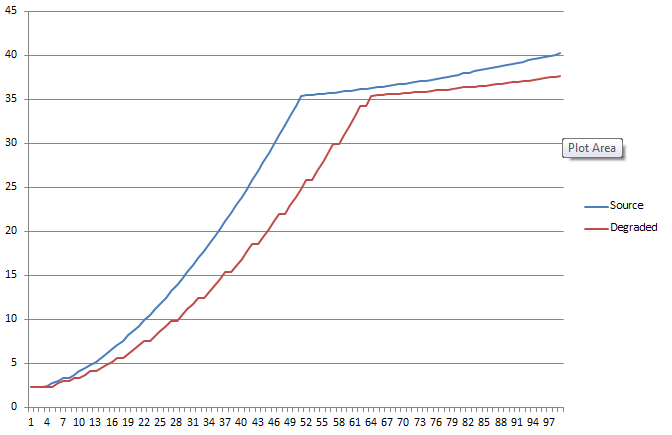
\includegraphics[width=.7\textwidth,natwidth=672,natheight=435]{images/stdDevEdgeImg.png}
	\caption{Source and degraded standard deviation edge image.}
	\label{fig:stdDevEdgeImg}
\end{figure}

Figure~\ref{fig:stdDevEdgeImg} visualizes the values from the standard deviation of the Sobel Filter edge image. In this test we used a source video sequence at 24 frames per second and a degraded signal at 30 frames per second. We see that the degraded signal is lagging behind the source signal more and more, and that the standard deviation value is completely similar for two consecutive frames each time the degraded signal seems to be additionally delayed. While this is just a small part of the PEVQ model, the standard deviation from the edge image, among other results, is used to perform the coarse temporal alignment as described in section~\ref{sect:pevq}. The result from figure~\ref{fig:stdDevEdgeImg} clearly illustrates that the video sequence will need some sort of temporal alignment in order for the two video sequences to be properly aligned. If such an alignment is not performed, further analysis on a frame by frame basis will not match in the time domain.  With regards to what we talked about in section~\ref{sect:coding}, this discovery translates to the fact that we need to run the alignment module. 

%%%%%%%%%%%%%%%%%%%%%%%%%%%%%%%%%%%%%%%%%%%%%%%%%%%%%%%%%%%%%%%%%%%
%%%%%%%%%%%%%%%%%%%%%%%%%% S U M M A R Y %%%%%%%%%%%%%%%%%%%%%%%%%%
%%%%%%%%%%%%%%%%%%%%%%%%%%%%%%%%%%%%%%%%%%%%%%%%%%%%%%%%%%%%%%%%%%%

\section{Summary}\label{sect:summary}
We have described today's situation with regards to objective video quality assessment, where available tools are either too expensive for most users, or provide results that correlates poorly with subjective test results. We have given an overview of the history of standardization of no-, reduced- and full-reference objective video quality assessment tools as well as a description of the difference between these approaches. Based on the test results of the standardized models we have argued for why we have chosen the PEVQ model which we will implement, and we have given a brief description of design decisions and plans for our own implementation. Finally we have given an overview of our current progress on the implementation, including a description of the results it provides when testing a video sequence with certain degradation.

\subsection{Future work}\label{sect:future work}
The main goal and what we will begin working on is implementing the PEVQ model exactly as it is described in the standardization ITU-T Rec. J.247. This work has begun, and will continue over the last half of 2015. As mentioned in section~\ref{sect:cts} the standardized PEVQ model we are implementing does not support HD resolution. Another research topic we must keep in mind once our implementation is done is therefore extending our solution to support resolutions above VGA. We also mentioned in~\ref{sect:coding} that speedup using a Graphics Processing Unit(GPU) can potentially be significant, and we would like to look at the possibility of performing parts of the calculation in the PEVQ model on a GPU.

\subsection{Related Work}\label{sect:related work}

\textit{``Background and related work'':} where you describe the
  scenario in more detail, the requirements, desired functionality,
  etc. Then, you describe related work and evaluate it against your
  requirements and hopefully can conclude that you need something new,
  which you describe in the next chapter

\subsubsection{PSNR}\label{sect:related work psnr}
	lots of stuff to say about psnr. Cheapasses use it etc.

\chapter{Background}                  


%%%%=========================================%%%%
%%%%=========================================%%%%
%%%%=========================================%%%%
\part{The project}                   
%%%%=========================================%%%%
%%%%=========================================%%%%
%%%%=========================================%%%%

% Uncertain if i need this. Perhaps just use "Choosing the standard"
\chapter{Planning the project} 

\section{Existing Tools}
PSNR, or pay to use tools, such as those standardized which we will look at in section \ref{sect:choosing the standard}

\section{Choosing the Standard}\label{sect:choosing the standard}

\subsection{The ITU-T J.247 Full Reference Models}
J.247 includes 4 possible models for full reference testing. A detailed explanation of all the models are published in ITU-T J.247 which makes it possible to implement all of these models. The models are however only tested for CIF (352x248), QCIF (176x144) and VGA (640x480) resolutions which is a limiting factor as these are all low resolutions compared to HD which is most used today (gonna need something more/better to say about this).

\subsubsection{NTT Full Reference Method}
Overall lowest scores among the 4 models described in J.247.

\subsubsection{OPTICOM's PEVQ Model}
High scores on average. 

\subsubsection{Psytechnics Full Reference Method}
High scores, but some drops in correlation with subjective test results where the OPTICOM model scores are more even.


\subsubsection{Yonsei University Full Reference Method}
Some really high scores, but otherwise more low scores.

\subsection{The ITU-T J.342 HDTV Full Reference Standard}
An updated version of OPTICOMs PEVQ model standardized in ITU-T J.247. Made for HD, more relevant today. However is published with code and copyrighted. The model is also more complex(?).

\subsection{Choosing OPTICOM's PEVQ Model from ITU-T J.247}
Standardized, (almost) no copyrights/patents. Overall most consistent results.

\chapter{Initial Implementation of PEVQ}
After having chosen OPTICOM's PEVQ model for our initial implementation we begun by getting an overview of the model. When we had a fair understanding of the work that had to be done to create an implementation we researched the various possible languages the model could be implemented with, what platforms it should run on, as well as what libraries may be of use during the implementation.

\subsection{Platforms, Coding Language and Third Party Libraries}
We had wish from the beginning that our solution would run on the three major operating systems available today; Microsoft Windows, Mac OS and Linux. In addition, as the PEVQ model contain a large amount of heavy computation, we felt it was important to create the implementation in a language where we as programmers have a large variety of optimization possibilities available. Our initial understanding of PEVQ made us realize that the majority of the execution time for an implementation would be spent performing image filtering operations on a per pixel basis. We believed these operations to be perfect for parallelization, perhaps even using a Graphics Processing Unit (GPU) at a later stage.

Based on these wishes we decided either C or C++ would be a good choice. Both languages gives the programmer the ability develop structured code with low level optimizations. There are also a large amount of third party APIs available for both languages which could help during the development, and both languages can be used for GPU programming. 

Out of these two possibilities we chose C++ as we both wanted to write an object oriented implementation, and we both had previous experience programming with the language. 

In addition to using C++ we wanted to use a library for video encoding. It was not relevant for our work to write our own video encoding, and it would have been 



\chapter{Testing the Initial Implementation}
       


\chapter{Rewriting the Initial Implementation}
Unclear when to use full sequence length and when to use stopMatch - startMatch. We decided to always use full video length (max(srcLen, degLen)), and use start and stop match as range within the respective array/matrix.

%%--------



%%%%=========================================%%%%
%%%%=========================================%%%%
%%%%=========================================%%%%
\part{Conclusion}  
%%%%=========================================%%%%
%%%%=========================================%%%%
%%%%=========================================%%%%
                  
\chapter{Conclusion}\label{chap:concl}

Here are some ideas for the conclusion.

%%%%%%%%%%%%%%%%%%%%%%%%%%%%%%%%%%%%%%%%%%%%%%%%%%%%%%%%%%%%%%%%%%%
%%%%%%%%%%%%%%%%%%%%%%%%%%%%%%%%%%%%%%%%%%%%%%%%%%%%%%%%%%%%%%%%%%%
%%%%%%%%%%%%%%%%%%%%%%%%%%%%%%%%%%%%%%%%%%%%%%%%%%%%%%%%%%%%%%%%%%%
\section{Summary}

In this section, you typically write about wyat you have done to
address the problem statement in section~\ref{sect:prob-statement}.


%%%%%%%%%%%%%%%%%%%%%%%%%%%%%%%%%%%%%%%%%%%%%%%%%%%%%%%%%%%%%%%%%%%
%%%%%%%%%%%%%%%%%%%%%%%%%%%%%%%%%%%%%%%%%%%%%%%%%%%%%%%%%%%%%%%%%%%
%%%%%%%%%%%%%%%%%%%%%%%%%%%%%%%%%%%%%%%%%%%%%%%%%%%%%%%%%%%%%%%%%%%
\section{Main Contributions}

Mainly repeat the content from section \ref{sect:contributions}:
List your main achievements here. Main results and what kind of
conclusions can be drawn...!? What new knowledge has been found!?
 
%%%%%%%%%%%%%%%%%%%%%%%%%%%%%%%%%%%%%%%%%%%%%%%%%%%%%%%%%%%%%%%%%%%
%%%%%%%%%%%%%%%%%%%%%%%%%%%%%%%%%%%%%%%%%%%%%%%%%%%%%%%%%%%%%%%%%%%
%%%%%%%%%%%%%%%%%%%%%%%%%%%%%%%%%%%%%%%%%%%%%%%%%%%%%%%%%%%%%%%%%%%
\section{Future work}

What is still missing that you see could be done, e.g., new
experiments, more functionality, comparison agains other systems,
optimizations of the code, ...


\chapter{Results}                     %% ... or ??


\chapter{Latex testing} 

This is some text referring to some code in \cref{code:testCode}. Lorum Ipsum etc etc dnu. just need to fill some lines of tex so it alll loooooks greaaaaat.

\codebox{%
%listing and comment, % Override default value (listing only)
%comment={The code in the Linux kernel that determines if a stream is thin},
label={code:testCode},
}
/* Testing a comment before the code */
void CoarseTemporalAlignment::realign(cv::Mat src, cv::Mat &dst, int numFrames){
    dst = cv::Mat::zeros(src.rows, src.cols, src.type());
    cv::Mat srcRoi;
    if (numFrames >= 0) {
        srcRoi = src(cv::Rect(0, 0, src.cols - numFrames, src.rows));
        srcRoi.copyTo(dst(cv::Rect(numFrames, 0, dst.cols - numFrames, dst.rows)));
    } else {
        srcRoi = src(cv::Rect(-numFrames, 0, src.cols + numFrames, src.rows));
        srcRoi.copyTo(dst(cv::Rect(0, 0, dst.cols + numFrames, dst.rows)));
    }
\end{cppcode}
\boxcaption{codelisting}{Test caption etc etc}

This is testtext for referencing a missing figure. Now im refereing it here \cref{figure:missingFigureTest}. That was it.
\begin{figure}%[H]
\centering
\begin{figurebox}[label={figure:missingFigureTest}]
\missingfigure{Showing that i miss a figure right here!}
\end{figurebox}
\caption{Missing figure caption.}
\end{figure}



\acomment{Testing acomment or something}

\atodo[inline]{Inlined atodo note aparently}
\atodo{none inlined atodo note?}

\citeneeded[inline]{Inlined citeneeded.}
\citeneeded{None-inlined citeneeded}

\backmatter{}
\bibliographystyle{unsrt}
\bibliography{all}
\end{document}

